% Options for packages loaded elsewhere
\PassOptionsToPackage{unicode}{hyperref}
\PassOptionsToPackage{hyphens}{url}
%
\documentclass[
]{article}
\usepackage{amsmath,amssymb}
\usepackage{lmodern}
\usepackage{ifxetex,ifluatex}
\ifnum 0\ifxetex 1\fi\ifluatex 1\fi=0 % if pdftex
  \usepackage[T1]{fontenc}
  \usepackage[utf8]{inputenc}
  \usepackage{textcomp} % provide euro and other symbols
\else % if luatex or xetex
  \usepackage{unicode-math}
  \defaultfontfeatures{Scale=MatchLowercase}
  \defaultfontfeatures[\rmfamily]{Ligatures=TeX,Scale=1}
\fi
% Use upquote if available, for straight quotes in verbatim environments
\IfFileExists{upquote.sty}{\usepackage{upquote}}{}
\IfFileExists{microtype.sty}{% use microtype if available
  \usepackage[]{microtype}
  \UseMicrotypeSet[protrusion]{basicmath} % disable protrusion for tt fonts
}{}
\makeatletter
\@ifundefined{KOMAClassName}{% if non-KOMA class
  \IfFileExists{parskip.sty}{%
    \usepackage{parskip}
  }{% else
    \setlength{\parindent}{0pt}
    \setlength{\parskip}{6pt plus 2pt minus 1pt}}
}{% if KOMA class
  \KOMAoptions{parskip=half}}
\makeatother
\usepackage{xcolor}
\IfFileExists{xurl.sty}{\usepackage{xurl}}{} % add URL line breaks if available
\IfFileExists{bookmark.sty}{\usepackage{bookmark}}{\usepackage{hyperref}}
\hypersetup{
  pdftitle={Codebook bundeslaendeR Government Data},
  pdfauthor={Robert Stelzle},
  hidelinks,
  pdfcreator={LaTeX via pandoc}}
\urlstyle{same} % disable monospaced font for URLs
\usepackage[margin=1in]{geometry}
\usepackage{graphicx}
\makeatletter
\def\maxwidth{\ifdim\Gin@nat@width>\linewidth\linewidth\else\Gin@nat@width\fi}
\def\maxheight{\ifdim\Gin@nat@height>\textheight\textheight\else\Gin@nat@height\fi}
\makeatother
% Scale images if necessary, so that they will not overflow the page
% margins by default, and it is still possible to overwrite the defaults
% using explicit options in \includegraphics[width, height, ...]{}
\setkeys{Gin}{width=\maxwidth,height=\maxheight,keepaspectratio}
% Set default figure placement to htbp
\makeatletter
\def\fps@figure{htbp}
\makeatother
\setlength{\emergencystretch}{3em} % prevent overfull lines
\providecommand{\tightlist}{%
  \setlength{\itemsep}{0pt}\setlength{\parskip}{0pt}}
\setcounter{secnumdepth}{-\maxdimen} % remove section numbering
\usepackage{longtable}
\usepackage{float}
\usepackage{graphicx}
\usepackage{booktabs}
\usepackage{longtable}
\usepackage{array}
\usepackage{multirow}
\usepackage{wrapfig}
\usepackage{float}
\usepackage{colortbl}
\usepackage{pdflscape}
\usepackage{tabu}
\usepackage{threeparttable}
\usepackage{threeparttablex}
\usepackage[normalem]{ulem}
\usepackage{makecell}
\usepackage{xcolor}
\ifluatex
  \usepackage{selnolig}  % disable illegal ligatures
\fi

\title{Codebook bundeslaendeR Government Data}
\author{Robert Stelzle}
\date{15 1 2022}

\begin{document}
\maketitle

\hypertarget{ltw_election_results_and_governments}{%
\subsection{\texorpdfstring{\texttt{ltw\_election\_results\_and\_governments}}{ltw\_election\_results\_and\_governments}}\label{ltw_election_results_and_governments}}

This codebook only concerns variables specific to the
\texttt{ltw\_election\_results\_and\_governments} dataset. For further
variables plese refer to the \texttt{ltw\_election\_results} dataset's
codebook.

\texttt{ltw\_election\_results\_and\_governments} returns a returns data
frame (tibble if the tibble package is loaded) containing both election
results as well as linked information on governments in the German
states. Each row contains information on one party during the time in
office of one cabinet.

Election results data are provided by the Bundeswahlleiter. A
machine-readable version of the data in the pdf available here
(\url{https://www.bundeswahlleiter.de/service/landtagswahlen.html}) was
kindly provided to me. Election data outside the timeframe covered by
Bundeswahlleiter's data provided to me was collected from the states'
local election authorities' (Landeswahlleiter) websites. More
information on parties and the continuity of parties under different
labels was collected by me. Information on Governments mainly taken from
the replication data of Linhart, Eric, Franz U. Pappi und Ralf Schmitt
(2008): Die proportionale Ministerienaufteilung in deutschen
Koalitionsregierungen: Akzeptierte Norm oder das Ausnutzen strategischer
Vorteile?, Politische Vierteljahresschrift 49(1): 46-67. To be found
online here:
\url{https://www.tu-chemnitz.de/phil/politik/pspi/forschung/daten.php}.
Information outside the timeframe of Linhart et al.~as well as
information on the names and party affiliations of the
Ministerpräsidenten was collected by me, mainly from German Wikipedia.

\begin{longtable}{p{3.2cm}| p{11cm}}
\texttt{gov\_no\_within\_
legterm} &\textbf{Number of cabinet within legislative term}\newline 
Number of cabinet within legislative term (i.e. First cabinet in the 1990-1994 legislative term of state X).



\hspace*{.25cm}
\begin{minipage}[t]{\linewidth }
\vspace{0pt}
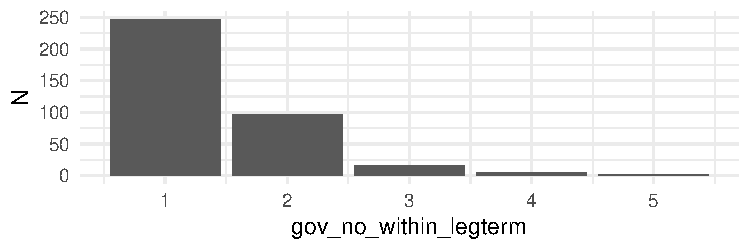
\includegraphics[width = \linewidth]{cbgov/govnolegperplot.pdf}
\end{minipage}



\end{longtable}

\begin{longtable}{p{3.2cm}| p{11cm}}
\texttt{gov\_id} &\textbf{Government ID}\newline 
Unique ID of government. Taken from Linhart et al. However, this ID is not counting up within state by time. In cases where Governments were 
           missing from Linhart et al. before the timeframe covered by Linhart et al. (eg. in Berlin) these earlyer governments have an higher ID than later cabinets 
           contained in Linhart et al. data.
\end{longtable}

\begin{longtable}{p{3.2cm}| p{11cm}}
\texttt{state\_gov\_
number} &\textbf{Number of government in state.}\newline 
Number of government in state.



\hspace*{.25cm}
\begin{minipage}[t]{\linewidth }
\vspace{0pt}
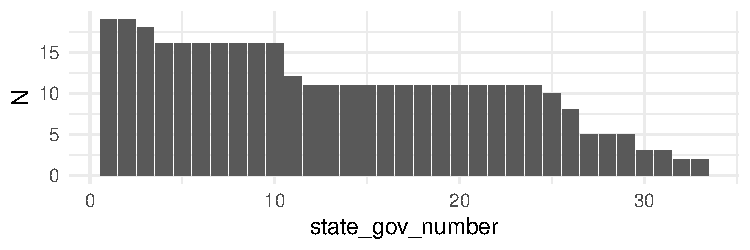
\includegraphics[width = \linewidth]{cbgov/stategovnumplot.pdf}
\end{minipage}



\end{longtable}

\begin{longtable}{p{3.2cm}| p{11cm}}
\texttt{gov\_party} &\textbf{Government Party}\newline 
Boolean wether the party was a cabinet party. Note: There is a single cabinet where no party is marked as part of the cabinet: Heinrich Welsch's caretaker government in the Saarland (at the time not yet a member of the FRG) in 1955.
\end{longtable}

\begin{longtable}{p{3.2cm}| p{11cm}}
\texttt{nmin\_party} &\textbf{Number of Ministers of Party}\newline 
Number of Ministers of Party.



\hspace*{.25cm}
\begin{minipage}[t]{\linewidth }
\vspace{0pt}
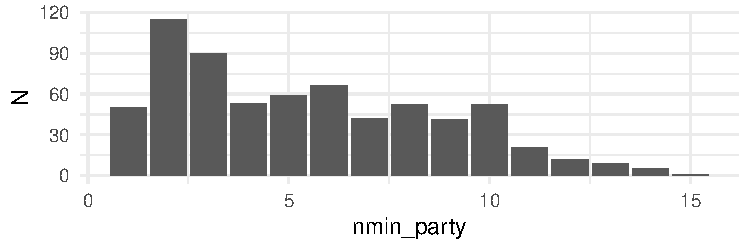
\includegraphics[width = \linewidth]{cbgov/nminpartyplot.pdf}
\end{minipage}



\end{longtable}

\begin{longtable}{p{3.2cm}| p{11cm}}
\texttt{gov\_source} &\textbf{Government Source}\newline 
Source of the information on the government. Either Linhart et al. or the URL of the German Wikipedia Page containing information on the cabinet.
\end{longtable}

\begin{longtable}{p{3.2cm}| p{11cm}}
\texttt{gov\_remarks\_
stelzle} &\textbf{Governments remarks Stelzle}\newline 
My remarks on governments.
\end{longtable}

\begin{longtable}{p{3.2cm}| p{11cm}}
\texttt{minister\_president} &\textbf{Name of minister president}\newline 
Name of minister president.
\end{longtable}

\begin{longtable}{p{3.2cm}| p{11cm}}
\texttt{mp\_party} &\textbf{Minister President's Party}\newline 
Party of the minister president. partyname\_short format used. Note: There is a single cabinet with an independent minister president: Heinrich Welsch's caretaker government in the Saarland (at the time not yet a member of the FRG) in 1955.
\end{longtable}

\begin{longtable}{p{3.2cm}| p{11cm}}
\texttt{is\_mp\_party} &\textbf{Is MP Party?}\newline 
 the governments minister president from this party? Note: There is a single cabinet where the minister president is not part of any party: Heinrich Welsch's caretaker government in the Saarland (at the time not yet a member of the FRG) in 1955.
\end{longtable}

\end{document}
